\documentclass[
 manuscript=article,  %% article (default),SpecialIssue,data,software,editorial
  layout=publish, 
  year=2024, 
  month= Februari, %check cls jika dibutuhkan
  volume=8,
  number=1 
]{JIKO}
\usepackage{hyphenat} 
%%%%++++++++++++++++++++++
\hyphenation{
	soft-ware 										
	di-la-ku-kan 
	di-la-kukan 
	me-nam-bah-kan
	meng-gu-na-kan
}
%%%%++++++++++++++++++++++
\usepackage{algorithm,algpseudocode}
\usepackage{courier,multirow,multicol}
\usepackage{listings}
\usepackage[bahasa,english]{babel}
\usepackage{blindtext}

\lstset{basicstyle=\ttfamily \small , language=python} 
\lstset{basicstyle=\ttfamily \small, language=html}
\lstset{basicstyle=\ttfamily \small, language=c++}

\doi{10.26798/jiko.}

%%%%%%%%%%%%%%%%%%%%%%%%%%%%%%%%%%%%%%%%%%%%%%
%%											%%
%%				RIKIE - UTDI- 				%%
%%											%%
%%%%%%%%%%%%%%%%%%%%%%%%%%%%%%%%%%%%%%%%%%%%%%

\newcommand{\id}{xxx} %Sesuaikan dengan ID Artikel
\setcounter{page}{15}  %Halaman pertama



\frenchspacing

% --- AREA AUTHOR ---
% Pastikan Judul artikel tidak lebih dari 12 kata
\title{%
	Analisis Perbandingan GraphQL dan REST API pada Aplikasi Menu Restoran dengan Node.js\\
	% {\large Sub-judul jika diperlukan}\\[1ex]
	\itshape Comparative Analysis of GraphQL and REST API in Node.js-Based Restaurant Menu Applicationsh\\
	% {\large Subtitle if needed in English}%
}

\newcommand{\judul}{Judul Dalam Bahasa Indonesia-Sub-judul jika diperlukan}

\author{Agung Prasetyo}
\email{agung.prasetyo@students.utdi.ac.id} %---> pindahkan email ini dibawah author korespondensi.
% \newcommand{\refnama}{M. I. Alharits} %Pastikan ini benar
\affiliation{Teknik Komputer, Fakultas Teknologi Informasi, Universitas Teknologi Digital Indonesia, Yogyakarta, Indonesia}


\author{Danny Kriestanto}
\affiliation{Departmen, Fakultas, Kampus-2, Kota, Negara}

% \author{Penulis Ketiga}
% \affiliation{Departmen, Fakultas, Kampus-1, Kota, Negara}
% \email{correspondence@email.ac.id} %---> pindahkan email ini dibawah author korespondensi.

%------------------------------------ penambahan author
% \author{Penulis Keempat}
% \affiliation{Departmen, Fakultas, Kampus-4, Kota, Negara}

\received{22-11-24}
\accepted{23-3-24}
\published{30-3-24}



% Mkasimum 5 Kata dalam keywords
\keywords{Kata kunci: Perbandingan; GraphQL; REST API; Node.js; K6 } 

\keywordsing{KeyWords: Comparison; GraphQL; REST API; Node.js; K6 } 
% Penting, hanya indeks singkatan jika istilah berisi lebih dari dua kata, dan istilah tersebut digunakan lebih dari sepuluh kali di seluruh makalah. Jika tidak, uraikan secara lengkap di dalam artikel.


\begin{document}
%\begin{CJK*}{UTF8}{gbsn}

%%%%%%%%%%%%%% ABSTRAK %%%%%%%%%%%%%%%%%%%%%%%%%%%%
 
\begin{abstract}
Penelitian ini bertujuan untuk menganalisis perbandingan performa antara GraphQL dan REST API pada aplikasi menu restoran berbasis Node.js, dengan fokus pada aspek waktu respons, penggunaan bandwidth, dan fleksibilitas. Masalah yang diangkat adalah menentukan solusi API yang optimal untuk aplikasi yang membutuhkan pengelolaan data secara efisien dan cepat. Pengujian dilakukan di lingkungan cloud menggunakan layanan gratis untuk menggambarkan kondisi nyata. Pendekatan penelitian dilakukan dengan pengujian performa menggunakan K6, alat yang digunakan untuk mensimulasikan beban permintaan pada server. Parameter yang diukur meliputi jumlah total permintaan, rata-rata waktu respons, volume data yang diterima dan dikirim, serta stabilitas server di bawah beban tinggi. Hasil analisis menunjukkan bahwa waktu respons GraphQL dan REST API tidak berbeda secara signifikan. Namun, GraphQL memiliki keunggulan dalam efisiensi bandwidth, karena hanya mengirim data yang diminta oleh klien, sedangkan REST API cenderung kurang fleksibel dan menghasilkan pengiriman data berlebih yang tidak selalu diperlukan klien. Hasil penelitian ini menunjukkan bahwa GraphQL unggul dibandingkan REST API dalam hal efisiensi data, kestabilan performa, dan fleksibilitas pengambilan data. GraphQL lebih hemat bandwidth dan memberikan kontrol lebih besar kepada klien dalam memilih data yang dibutuhkan, menjadikannya pilihan terbaik untuk aplikasi dengan kebutuhan data dinamis dan skalabilitas tinggi. Namun, REST API tetap efektif untuk aplikasi dengan arsitektur sederhana yang tidak memerlukan kustomisasi data kompleks.
\end{abstract}

\begin{abstracting}
This study aims to analyze the comparative performance of GraphQL and REST API on a Node.js-based restaurant menu application, focusing on aspects of response time, bandwidth usage, and flexibility. The problem raised is to determine the optimal API solution for applications that require efficient and fast data management. Testing is carried out in a cloud environment using free services to describe the actual conditions. The research approach is carried out by testing performance using K6, a tool used to simulate the request load on the server. The parameters measured include the total number of requests, average response time, volume of data received and sent, and server stability under high load. The results of the analysis show that the response time of GraphQL and REST API is not significantly different. However, GraphQL has an advantage in bandwidth efficiency, because it only sends data requested by the client, while REST API tends to be less flexible and results in sending excessive data that is not always needed by the client. The results of this study indicate that GraphQL is superior to REST API in terms of data efficiency, performance stability, and flexibility of data retrieval. GraphQL is more bandwidth efficient and gives clients more control in choosing the data they need, making it the best choice for applications with dynamic data needs and high scalability. However, REST APIs remain effective for applications with simple architectures that do not require complex data customization..
\end{abstracting}
%%%%%%%%%%%%%%%%%%%%%%%%%%%% PENDAHULUAN %%%%%%%%%%%%%%%%

\section{Pendahuluan}
Perkembangan teknologi yang cepat telah menghadirkan berbagai metode baru untuk mengelola dan bertukar data antara \textit{backend} dan \textit{frontend}, terutama melalui \textit{Application Programming Interface} (API). Salah satu metode yang paling umum digunakan adalah \textit{Representational State Transfer} (REST), yang telah menjadi tulang punggung aplikasi web modern \cite{[1]}. Namun, seiring dengan meningkatnya kebutuhan untuk pengelolaan data yang lebih efisien, \textit{GraphQL} muncul sebagai alternatif yang lebih fleksibel, memungkinkan \textit{client} untuk menentukan dengan tepat data apa yang ingin diambil dari \textit{server} \cite{[2]}.

\textbf{REST API} sering menghadapi masalah \textit{over-fetching} dan \textit{under-fetching}. \textit{Over-fetching} terjadi ketika \textit{client} menerima lebih banyak data daripada yang dibutuhkan, sedangkan \textit{under-fetching} terjadi ketika \textit{client} tidak mendapatkan data yang cukup, sehingga memerlukan permintaan tambahan \cite{[3]}. Masalah ini bisa mempengaruhi performa aplikasi yang mengelola data kompleks, seperti memperlambat waktu respons dan meningkatkan penggunaan bandwidth.GraphQL hadir sebagai solusi dengan memungkinkan client meminta data yang lebih spesifik sesuai kebutuhan \cite{[4]}.

Sampai saat ini, telah dilakukan beberapa penelitian yang membahas perbandingan antara \textbf{REST API} dan \textbf{GraphQL API}. Pada penelitian sebelumnya, rata-rata \textit{REST API} masih mengungguli dari segi performa, namun untuk fleksibilitas permintaan data \textbf{GraphQL} bisa menjadi alternatif saat ini. Pada penelitian yang dilakukan penulis, penulis menggunakan lingkungan cloud dengan memanfaatkan layanan gratis. Merujuk pada penelitian sebelumnya sudah ada yang pernah mengulas topik ini menggunakan teknologi \textbf{Node.js}. Namun, kelemahannya adalah penelitian tersebut hanya menganalisis \textbf{HTTP Request} dalam lingkungan lokal.

Oleh karena itu berdasarkan fakta dan permasalahan di atas, penulis bertujuan untuk menganalisis terhadap kinerja \textbf{REST API} dan \textbf{GraphQL} yang diharapkan dapat membantu untuk menentukan arsitektur \textbf{API} yang terbaik dalam membangun sebuah aplikasi menggunakan teknologi \textbf{Node.js} pada lingkungan \textit{cloud}. \textit{Response time}, \textit{bandwidth usage}, dan fleksibilitas menjadi tolok ukur dalam penelitian ini \cite{[5]}. Semakin cepat waktu respons dalam memproses permintaan data dan mengembalikannya ke \textit{client}, semakin cepat pula informasi yang tersampaikan kepada pengguna. Hal ini berkontribusi langsung terhadap kepuasan pengguna web service, di mana waktu tunggu yang lebih rendah akan meningkatkan pengalaman pengguna secara keseluruhan.

%%%%%%%%%%%%%%%%%%%%%%%%%%%% METODE %%%%%%%%%%%%%%%%%%%%%%%%%%%%%
\section{Metode}

Penelitian ini dilakukan melalui beberapa tahapan yang bertujuan untuk membandingkan implementasi \textbf{GraphQL} dan \textbf{REST API} pada aplikasi menu restoran menggunakan \textit{Node.js}. Setiap tahapan dirancang secara sistematis untuk memastikan keluaran penelitian sesuai dengan harapan dan memberikan gambaran yang jelas mengenai performa kedua metode \textbf{API} dalam konteks yang diujikan. Tahapan penelitian ini meliputi:


\begin{figure}[ht!]
	\centering
	\subfloat[$\rho^2-\theta_1$ and $\rho^2-\theta_2$]{%
		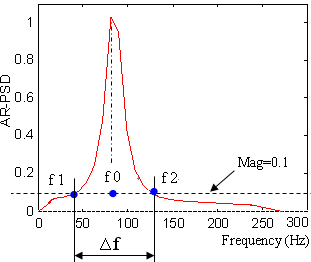
\includegraphics[width=0.25\textwidth]{3a.png}%
	}%
	\subfloat[$\delta_1-\theta_1$ and $\delta_1-\theta_2$]{%
		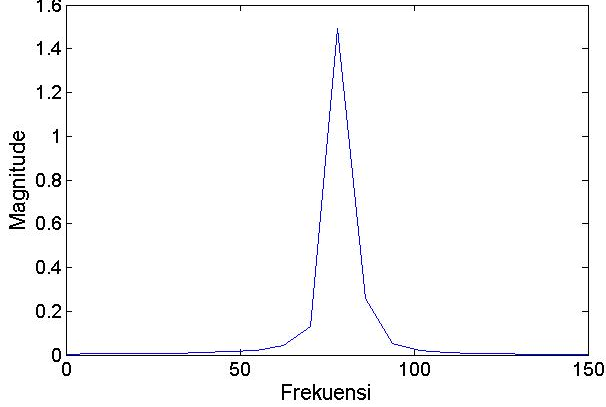
\includegraphics[width=0.3\textwidth]{3b.png}%
	}
	
	\subfloat[The variation of $\theta_1$ ]{%
		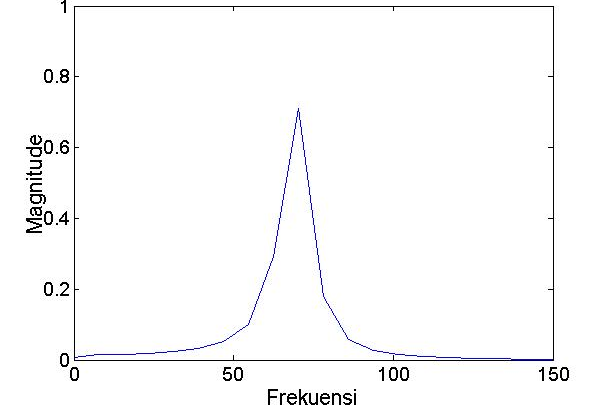
\includegraphics[width=0.3\textwidth]{3c.png}%
	}%
	\subfloat[The variation of $\rho^2$ and $\delta_1$]{%
		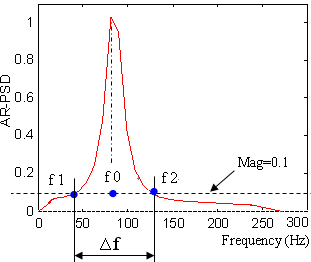
\includegraphics[width=0.25\textwidth]{3a.png}%
	}
	
	\medskip
	
	\begin{minipage}{0.9\textwidth}
		\small
		(a) dievaluasi pada $(\delta_0, \delta_1)=(0.1,0.01)$ dan $(\alpha,\beta)=(1,1)$, \\
		(b) dievaluasi pada $(\delta_0,\rho^2)=(0.1,1)$ dan $(\alpha,\beta)=(1,1)$, \\
		dan (c) (d) dievaluasi pada $\delta_0=0.1$ dan $(\alpha,\beta)=(1,1)$.
	\end{minipage}
	\medskip
	
	\caption{Variasi dari $\theta_1$ dan $\theta_2$ berkenaan dengan $\rho^2$ dan $\delta_1$} \label{subfigure}
\end{figure}


\subsection{Studi Literatur}

Pada tahap awal, dilakukan studi literatur untuk memahami konsep dasar \textbf{REST API} dan \textbf{GraphQL}, serta kelebihan dan kekurangan masing-masing metode. Selain itu, juga dilakukan kajian terhadap teknologi \textit{Node.js} yang akan digunakan sebagai platform pengembangan aplikasi. Informasi dari literatur ini akan menjadi dasar dalam mendesain sistem.

\subsection{Perancangan Sistem}

Tahap ini melibatkan perancangan aplikasi menu restoran yang akan diimplementasikan menggunakan dua metode \textbf{API}, yaitu \textbf{REST API} dan \textbf{GraphQL}. Desain sistem mencakup arsitektur aplikasi, struktur database, serta \textit{endpoint} \textbf{API} yang digunakan untuk mengakses data menu pada aplikasi menu restoran.


\subsection{Metode bagian 2 / subsection}


 Hasil akhirnya ada di Gambar \ref{fig:logo}. Tidak perlu memaksakan gambar berada pada halaman yang sama dengan naskah, cukup pastikan bahwa gambar dapat ditelusuri dengan baik walaupun berada pada halaman yang berbeda\cite{Erwi2015},\cite{Transport},\cite{soil-1-273-2015},\cite{article}.

\begin{figure}[ht!]
  \centering
  
\includegraphics[width=0.3\textwidth]{JIKOlogo.png}
  \caption{JIKO Logo}
  \label{fig:logo}
\end{figure}

\textbf{Ukuran gambar dapat diatur, tidak terlalu besar sehingga memakan banyak tempat, atau terlalu kecil sehingga tidak jelas dan sulit dibaca.}


Gunakan format tabel dibawah ini bila ingin memberikan catatan pada tabel, seperti terlihat pada Tabel~\ref{contohtabel}.
\begin{table}[hbt!]
	\begin{threeparttable}
		\caption{Sebuah Contoh Tabel dengan Keterangan tabel}
		\label{contohtabel}
		 \begin{tabular}{lll}
			\toprule
			\textbf{Parameter} & \textbf{Notation} & \textbf{Remarks} \\
			\midrule
			name & - & engine common identifier \\
			manufacture & - & name of the manufacture  \\
			bpr & $\lambda$ & bypass ratio \\
			pr & - & pressure ratio \\
			thrust & $T_0$ & maximum static thrust\\
			\bottomrule
		\end{tabular}

		\begin{tablenotes}[hang]
			\item[]Catatan
			\item[a]Catatan pertama
			\item[b]Catatan tabel lainnya.
		\end{tablenotes}
	\end{threeparttable}
\end{table}

\subsubsection{Metode bagian 2-1 / subsubsection }

Referensi ke Persamaan~\ref{eq:cauchy_momentum}, atau Anda dapat menggunakan format (eqref) persamaan~\eqref{eq:cauchy_momentum} untuk referensi persamaan.

\begin{equation}\label{eq:cauchy_momentum}
	d_{ij} = \sqrt{{\sum_{k=1}^{p}}(x_{ik}-y_{jk})^2}
\end{equation}

Dimana nilai dari:\\
\begin{tabular}{lcl}
	$d_{ij}$ &:& Jarak dari objek i dan objek j\\
	$P$		&:& Jumlah faktor dari cluster\\
	$x_{ik}$ 		&:& Data dari subjek i pada variable k\\
	$y_{jk}$ 		&:& Data dari subjek j pada variable k\\
\end{tabular}

Jangan lupa untuk menuliskan keterangan rumus Anda, baik notasi maupun keterangan lain yang diperlukan untuk memperjelas rumus yang Anda tulis.

Jika Anda menulis kode di artikel Anda, Anda dapat menuliskannya seperti contoh Koding~\ref{lst1} di bawah ini. Tidak masalah jika koding anda menggunakan bahasa selain bahasa inggris, tidak perlu ditulis miring, sesuaikan saja dengan koding yang anda buat.

\renewcommand{\lstlistingname}{Koding}
\begin{lstlisting}[
	caption={Contoh Koding bahasa html},label=lst1,language=html]
	
		<!DOCTYPE html>
		<html>
		<body>
		
		<h1>My First Heading</h1>
		<p>My first paragraph.</p>
		
		</body>
		</html>

\end{lstlisting}

Di bawah ini jika membutuhkan untuk metulis dalam bentuk algoritma, seperti terlihat pada Algoritma~\ref{alg1}:

\renewcommand{\algorithmname}{Algoritma}
\begin{algorithm}
	\caption{Sistem kontrol kelembaban tanah}\label{alg1}
	\begin{algorithmic}
		\State Inisialisasi dan kalibrasi sensor YL-69 dan mikrokontroler Arduino Mega 2560.
		\While{true}
		\State Ukur tingkat kelembapan tanah secara terus-menerus menggunakan sensor YL-69.
		\State Kirim data kelembaban tanah ke mikrokontroler untuk diproses.
		\If{tingkat kelembaban tanah  $<$ ambang batas}
		\State Aktifkan pompa air DC untuk menambahkan air ke tanah.
		\EndIf
		\State Menampilkan tingkat kelembaban tanah saat ini pada layar LCD 16x2.
		\EndWhile
		\State Ulangi langkah 2-6 secara terus menerus untuk menjaga tingkat kelembaban tanah yang tepat untuk pohon Gaharu.
	\end{algorithmic}
\end{algorithm}

\subsubsection{Metode bagian 2-2 / subsubsection}

Para penulis harus memastikan bahwa mereka telah menulis karya yang sepenuhnya asli, dan jika penulis telah menggunakan karya dan/atau kata-kata orang lain bahwa hal tersebut telah dikutip atau dikutip dengan tepat. 

\blindtext  

Table \ref{tb:example_table} menunjukkan sebuah contoh \cite{Johnson1962,articleLekshmi,Johnson1962,Rikie,Kolodzy}.

\begin{table}[H]
  \centering
  \small
  \caption{Contoh tabel}
  \label{tb:example_table}
  \begin{tabular}{lll}
  \toprule
  \textbf{Parameter} & \textbf{Notation} & \textbf{Remarks} \\
  \midrule
  name & - & engine common identifier \\
  manufacture & - & name of the manufacture  \\
  bpr & $\lambda$ & bypass ratio \\
  pr & - & pressure ratio \\
  thrust & $T_0$ & maximum static thrust\\
  \bottomrule
  \end{tabular}
\end{table}

Atau  dapat menggunakan tabel format lain (bukan untuk tabel panjang) seperti dapat dilihat di Tabel~\ref{standar}. Jika Anda harus menggunakan longtable, tambahkan \verb|\usepackage{longtable}| sebelum \verb|\begin{dokumen}| pada source \LaTeX, dan pastikan Anda tidak membuat longtable lebih dari 2 halaman.
\begin{table}[ht!]
	\centering
	\caption{Tabel standar, bukan longtable}
	\label{standar}
	\begin{tabular}{p{2cm}p{2cm}p{4cm}}\hline
		\textbf{Parameter} & \textbf{Notation} & \textbf{Remarks} \\\hline\hline
	 name & - & engine common identifier \\
	manufacture & - & name of the manufacture  \\
	bpr & $\lambda$ & bypass ratio \\
	pr & - & pressure ratio \\
	thrust & $T_0$ & maximum static thrust\\	\hline
	\multicolumn{3}{l}{{\scriptsize Sumber:\cite{Rikie}}}
	\end{tabular}
\end{table}

Jika anda membutuhkan tabel dengan multi-kolom dan multi-baris, anda dapat gunakan dan lihat contoh pada Tabel~\ref{multitab}, pastikan hanya menambahkan garis horizontal (selain pada header tabel dan akhir tabel) jika diperlukan untuk memperjelas tabel.  
\begin{table}[ht!]
	\centering \caption{Tabel multicol dan multirow} \label{multitab}
	\begin{tabular}{lllll}\hline
		\textbf{Head 1} & \textbf{Head 2} & \multicolumn{2}{c}{\textbf{Head 3}} & \textbf{Result}\\\hline\hline
		\multirow{2}{*}{1}& col2 & col3&col4& 123\\
		 & row2 & row2 & -- & 321\\ \hline
	\end{tabular}
\end{table}

	Anda dapat menambahkan Pustaka dalam bentuk \verb|\bibitem{citekey}| atau dengan menggunakan bib file. Pastikan anda menulis pustaka dengan baik dan menggunakan \textit{style IEEE}.

%%%%%%%%%%%%%%%%%%%%%%%%%%%%%%%%%%%%%%%%%% HASIL %%%%%%%%%%%%%%%%%%%%%%%%%%%%
\section{Hasil}

\paragraph{Paragraph title} Ini adalah paragraf dengan judul jika Anda ingin menggunakan fungsi tersebut di makalah \cite{Barden2000,Johnson1962,Kolodzy}. Harap jangan menyertakan konten yang berlebihan dan berulang di bagian ini. Khususnya, informasi yang diperoleh pembaca dari tabel, grafik, dll \cite{Rikie}.

Penting untuk memberikan informasi tentang metode statistik agar  dapat terus mengacu pada hasil penelitian dengan baik.
Mengenai uji statistik, informasi yang diperlukan seperti tingkat signifikansi, derajat kebebasan, dll harus disediakan, sedangkan rumus dan informasi terkait harus disebutkan di bagian metodologi\cite{Lutfiyana2017,Pramana2013,Wu}
Daripada memberikan banyak angka, lebih baik memberikan dalam bentuk rata-rata.

Ini menyediakan tabel, grafik, batang, dan lain-lain. Ini disajikan secara ringkas dan ringkas untuk membantu pembaca memahami topik dengan cepat dan jelas. Pastikan untuk menuliskan deskripsi grafik Anda, dan pastikan juga grafik Anda dapat terbaca dengan baik.
Hasil harus ditulis dalam urutan yang sesuai dengan urutan hipotesis.
Anda tidak boleh mencoba memperdebatkan alasan untuk menolak dan menerima hipotesis, tetapi serahkan pada bagian diskusi.
Jika temuan Anda dapat dijelaskan secara lengkap dalam beberapa kalimat teks, Anda tidak perlu menyertakan tabel.
 


%%%%%%%%%%%%%%%%%%%%%%%%%%%%%%%%%%%%%PEMBAHASAN %%%%%%%%%%%%%%%%%%%%%
\section{Pembahasan}

Mencoba memeras diskusi lengkap ke dalam satu paragraf dapat menambah tekanan yang tidak perlu pada proses penulisan. Jika memungkinkan, berikan dua atau tiga paragraf tambahan untuk memberi pembaca pemahaman yang komprehensif tentang studi Anda.\\
\textbf{Dalam paragraf pertama}, berikan interpretasi penting dari temuan kunci, dan sertakan bagian utama dari bukti pendukung.\\
\textbf{Paragraf kedua}, membandingkan dan membedakan dengan penelitian sebelumnya, dan menyoroti kekuatan dan keterbatasan penelitian. diskusikan temuan tak terduga.\\
\textbf{Dalam paragraf terakhir}, rangkum hipotesis dan tujuan penelitian, soroti pentingnya penelitian, dan diskusikan persamaan yang belum terjawab dan potensi penelitian di masa depan.

%%%%%%%%%%%%%%%%%%%%%%%%%%%%%%%%%%% SIMPULAN %%%%%%%%%%%%%%%%%%%%%%%%%
\section{Simpulan}

Nyatakan kembali topik penelitian Anda. Biasanya, satu kalimat cukup untuk menyatakan ulang topik dengan jelas, dan Anda akan menjelaskan mengapa topik Anda penting. Bagian dari kesimpulan Anda ini harus jelas dan ringkas dan hanya menyatakan informasi yang paling penting, jangan menuliskannya dalam bentuk numbering atau item, cukup \textbf{\textit{dalam paragraf utuh}}.

Anda dapat meringkas poin-poin utama penelitian Anda. Sangat membantu untuk membaca makalah Anda, memilih fakta dan argumen yang paling relevan. Anda tidak perlu menyertakan banyak informasi selain argumen atau fakta utama yang Anda sajikan dalam makalah Anda.

Setelah mendiskusikan poin-poin utama argumen Anda, Anda dapat mempresentasikan pentingnya poin-poin tersebut. Misalnya, setelah menyatakan poin utama yang Anda buat dalam argumen, Anda dapat mendiskusikan bagaimana dampak topik Anda memengaruhi hasil tertentu. Demikian pula, Anda dapat mempresentasikan hasil studi atau temuan lain yang dapat membantu menambah penekanan pada cara Anda mempresentasikan pentingnya informasi Anda.

Dapat pula memberikan rujukan \cite{Erwi2015,Rikie,Erwi2015}untuk untuk memperkuat simpulan anda. Jika ingin memberikan saran, berikan saran dengan mengacu pada apa yang menurut anda mungkin saja dilakukan dan berkaitan erat dengan hasil penelitian. Saran dalam artikel bersifat anjuran bukan sebuah keharusan\cite{Rikie,Kolodzy}.

%\appendix %Opsional jika Anda membutuhkannya


\section*{Sumber dana -- dianjurkan}
Berikan sumber pendanaan dari penelitian yang mendasari artikel ini.  
 
Crossmark yang ditampilkan di bawah logo JIKO, akan memberikan informasi metadata tentang artikel yang telah diterbitkan. 
 Meng-klik ikon CrossMark akan memberi informasi ke pembaca tentang status dokumen saat ini dan juga dapat memberikan informasi catatan publikasi tambahan tentang dokumen tersebut.

\section*{Ucapan Terima kasih}
Ucapkan terima kasih kepada mereka yang berperan aktif dalam penelitian dan penulisan karya Anda, jangan menulis terima kasih kepada orang yang tidak terlibat apa pun pada penelitian.
Tambahkan juga pernyataan pendanaan dari penelitian jika diperlukan.
\textbf{BAGIAN INI OPSIONAL}.

%%%%%%%%%%%%%%%%%%%%%%%%%%%%%%%%%%% PUSTAKA %%%%%%%%%%%%%%%%%%%%%%%%%%%%%%%
\section*{Tentang Referensi}
Pastikan anda telah menulis Referensi dengan benar menggunakan IEEE Style, dapat ditelusuri dan memiliki tingkat kesesuaian yang baik. Sangat dianjurkan pula lebih dari 90\% referensi anda adalah referensi primer, tuliskan link DOI artikel (sangat dianjurkan). Jangan menggunakan referensi lama, gunakan referensi terbaru (5 tahun terakhir) dan memiliki keterkaitan dengan artikel.

\renewcommand{\refname}{Pustaka} %%% nonaktifkan bila artikel bahasa inggris
	\bibliographystyle{IEEEtran}
\bibliography{reference}

%run it with pdflatex <file>, biber <file>, pdflatex <file>
% \begin{thebibliography}{00}

% 	\bibitem{1} G. R. D. T. Muntaner, “Evaluation of OpenFlow Controllers,” Tech. Rep., 2012. [Online]. Available:
% 	http://kth.diva-portal.org/smash/record.jsf?pid=diva2:563469
% 	\bibitem{2}D. Turull, M. Hidell, and P. Sjödin, “Performance evaluation of OpenFlow controllers for network virtualization,” High Perform. Switch. Routing (HPSR), 2014 IEEE 15th Int. Conf., pp. 50–56, 2014.
% 	\bibitem{3}G. Sdn and C. Testing, “ONOS Controller Performance Test Report,” Tech. Rep., 2016.
% 	\bibitem{4}I. T. S. Lab, “OpenDaylight Performance Stress Test Report,” Tech. Rep., 2016.ISSN: 2252-8776
% 	\bibitem{5}M. Sisov, “Building a Software-Defined Networking System with OpenDaylight Controller,” Ph.D. dissertation, Helsinki Metropolia University, 2016.
% 	\bibitem{6}S. Kaur, J. Singh, and N. Ghumman, “Network programmability using pox controller,” 08 2014.
% 	\bibitem{7}Yehdeya EF, Primasari CH, Sidhi TA, Wibisono YP, Setyohadi DB, Cininta M, "Analisis User Interface (UI) Dan User Experience (UX) Sudut Elevasi Pemukul Gamelan Metaverse Virtual Reality Menggunakan User Centered Design (UCD)", JIKO (Jurnal Informatika dan Komputer), 2023 Feb 6;7(1):137-46.
% 	\bibitem{8} A. Einstein, “Zur Elektrodynamik bewegter Körper. (German) [On the electrodynamics of moving bodies],”
% 	Annalen der Physik, vol. 322, no. 10, pp. 891–921, 1905.
% 	\bibitem{9} P. A. M. Dirac, The Principles of Quantum Mechanics, ser. International series of monographs on physics.
% 	Clarendon Press, 1981.
% 	\bibitem{10} R. E. Sorace, V. S. Reinhardt, and S. A. Vaughn, “High-speed digital-to-RF converter,” U.S. Patent
% 	5 668 842, Sep. 16, 1997.
% 	\bibitem{11} M. Yajnik, S. B. Moon, J. Kurose, and D. Towsley, “Measurement and modeling of the temporal depen-
% 	dence in packet loss,” in Proc. IEEE INFOCOM’99, vol. 1, New York, NY, Mar. 1999, pp. 345–352.
% 	\bibitem{12} N. C. Loh, “High-resolution micromachined interferometric accelerometer,” Master’s thesis, Massachu-
% 	setts Institute of Technology, Cambridge, 1992.
% 	\bibitem{13} Q. Li, “Delay characterization and performance control of wide-area networks,” Ph.D. dissertation, Univ.
% 	of Delaware, Newark, May 2000. [Online]. Available: http://www.ece.udel.edu/~qli
% 	\bibitem{14}R. Hidayati, A. Zubair, A. H. Pratama, and L. Indana, “Analisis Silhouette Coefficient pada 6 Perhitungan Jarak K-Means Clustering,” Techno.Com, vol. 20, no. 2, Art. no. 2, May 2021, doi: 10.33633/tc.v20i2.4556.
% 	\bibitem{15} R. Kartadie, F. Rozi, and E. Utami, “Openflow switch software-based performance test on its implementation on campus network,” Journal of Theoretical and Applied Information Technology, vol. 96, pp.
% 	4136–4146, 07 2018.
% 	\bibitem{16} J. P. Duque, D. D. Beltrán, and G. P. Leguizamón, “OpenDaylight vs . Floodlight : Comparative Analysis
% 	of a Load Balancing Algorithm for Software Defined Networking,” vol. 10, no. 2, pp. 348–357, 2018.
% 	\bibitem{17} S. Asadollahi and B. Goswami, “Experimenting with Scalability of Floodlight Controller in Software	Defined Networks,” in Int. Conf. Electr. Electron. Commun. Comput. Optim. Tech. Exp., no. December,
% 	2018, pp. 288–292.
% \end{thebibliography}

%\end{CJK*}
\end{document}
